\chapter{Optimización del firmware de los electroestimuladores}
En el presente capítulo se procede al estudio y mejora del firmware de los electroestimuladores de la prótesis híbrida. Se desea obtener un firmware optimizado en cuanto velocidad y eficiencia de comunicación con el exterior. Esto se debe a la necesidad de la rapidez por parte de los mismos para modificar parámetros de estimulación durante la realización de los ejercicios de rehabilitación.
\\
\\
Al igual que en el capítulo anterior, se identificarán los objetivos de mejora, en este caso del firmware, para poder plantear así tareas dedicadas a su mejora y optimización.
\\
\\
Por último, se validará el cumplimiento de las tareas mencionadas para culminar en una comparación de las versiones del firmware original y optimizada.

\section{Revisión del firmware y planteamiento de objetivos de mejora}
Tal y como se ha explicado en el capítulo \ref{capitulo_2} el electroestimulador mini TEREFES es capaz de comunicarse con el exterior mediante interrupciones por USART. De este modo, puede recibir comandos como el siguiente:

$$w\;0\;ap\;30\;\textbackslash r$$

lo cual significa escribir en el canal cero una amplitud de pulso positiva de 30$mA$.
\\
\\
Estos comandos se reciben como cadenas de caracteres lo que la instrucción anterior consta de diez, incluyendo espacios y el retorno de carro ($\textbackslash r$) para indicar el final de comando. Además, es necesario considerar que cada carácter tiene un tamaño de 1 byte por lo que el comando expuesto ocupa 10 bytes. Esto es importante debido a que los Registros de Datos del USART o UDR del microntrolador tienen un tamaño de 1 byte. Estos registros son los encargados de almacenar los datos que se reciben (registro de recepción) o transmiten (registro de transmisión) a través del puerto serie. En el caso se utiliza el USART1 por lo que sus registros de datos son UDR1 (los registros de transmisión y recepción comparten a misma dirección de entrada/salida o Input/Output. Cuando se escriben datos en UDR1 se almacenan en el registro de transmisión mientras que si se efectúa una lectura de UDR1 se accede al contenido del registro de recepción.) Se aprecia en la figura \ref{fig:USART_datasheet} la descripción del registro de datos del USART según la hoja de datos del ATmega128L.\\

\begin{figure}[!htb]
\centering
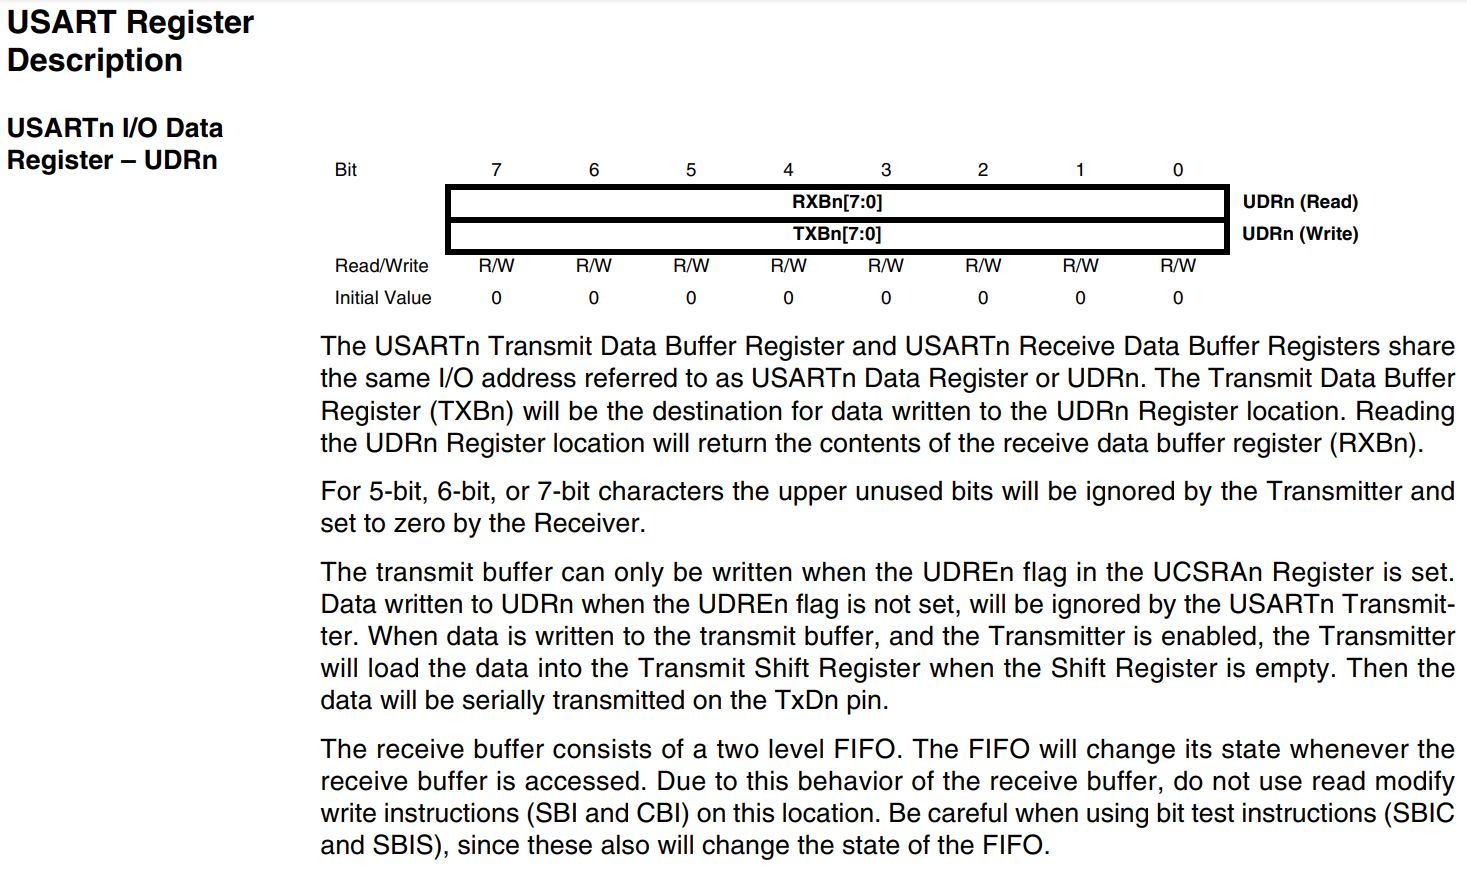
\includegraphics[scale=0.45]{USART_datasheet}
  \caption{Descripción del registro de datos asociado al USART del ATmega128L según su hoja de datos.}\label{fig:USART_datasheet}
\end{figure}

Analizando la la instrucción anterior que sirve de ejemplo, se observa que la forma de transmitir comandos al electroestimulador está implementada a alto nivel, es decir de cara al usuario que los transmite mediante una terminal y una conexión al puerto serie virtual correspondiente, tal y como se explicó en el capítulo \ref{capitulo_2}. El control de los estimuladores eléctricos en la prótesis híbrida requiere que el microcontrolador que sirve de nodo central efectúe la comunicación con estos dispositivos. Esto implica un control a un nivel más bajo, es decir, el usuario no tendrá contacto directo con estos comandos los cuales serán interpretados por el microcontrolador central para efectuar las correspondientes acciones. Incluso los datos solicitados a los estimuladores en cuanto a sus parámetros serán interpretados por la interfaz gráfica para mostrarlos por pantalla de la forma adecuada. 
\\
\\
Se puede ver cómo la implementación de los comandos en alto nivel deja de ser necesaria. Además, ésta presenta la principal desventaja que concierne al tamaño de los paquetes de datos que se transmiten y lo que en última instancia, influye a la velocidad de ajuste de parámetros de estimulación y la eficiencia en la asistencia durante la rehabilitación. Además, si un solo carácter se pierde o altera durante la comunicación, la instrucción completa será erróena.
\\
\\
Por lo tanto, el principal objetivo de mejora del firmware del estimulador es la codificación de instrucciones que recibe el mini TEREFES para que queden a un nivel más bajo y la comunicación sea más eficiente. 


\section{Codificación de instrucciones del estimulador eléctrico}
Para la tarea de codificación de instrucciones ha de considerar como factor limitante el tamaño del Registro de Datos del USART UDR1. Esto implica necesariamente trabajar con paquetes de datos de 1 byte ya que el microcontrolador no puede recibir o envíar más bytes de una vez. Cabe la posibilidad de utilizar 9 bits para datos pero esto no es compatible con todos los dispositivos que se puedan conectar con el estimulador, por lo que se mantiene la configuración original.
\\
\\
Antes de entrar en la codificación de instrucciones, se va a mostrar la totalidad de comandos que puede recibir el estimulador eléctrico. Estas instrucciones se muestran en la tabla \ref{tabla:comandos_originales}

\begin{table}
  \begin{tabular}{| c | c | c |}
      \hline
      \thead{Instrucción} & \thead{Valor numérico} & \thead{Descripción} \\
      \hline
      w <valor 1> ap <valor 2> &  \makecell{valor 1: [0,3]\\valor 2: [0,50]$mA$} & \makecell{Configuración de la amplitud de pulso positivo\\ recogida en el valor 2 para el canal\\ indicado por el valor 1.}  \\
      \hline
      w <valor 1> an <valor 2> &  \makecell{valor 1: [0,3]\\valor 2: [0,50]$mA$} & \makecell{Configuración de amplitud de pulso negativo\\ recogida en el valor 2 para el canal\\ indicado por el valor 1.}  \\
      \hline
      w <valor 1> re <valor 2> &  \makecell{valor 1: [0,3]\\valor 2: [0,3]} & \makecell{Configuración del número de repeticiones \\de pulso indicadas en valor 2\\ para el canal recogido en valor 1.} \\
      \hline
      w <valor 1> tp <valor 2> &  \makecell{valor 1: [0,3]\\valor 2: [250,500]$\mu s$} & \makecell{Configuración del ancho de pulso positivo\\ recogido en el valor 2 para el canal\\ indicado por el valor 1.}\\
      \hline
      w <valor 1> tn <valor 2> &  \makecell{valor 1: [0,3]\\valor 2: [250,500]$\mu s$} & \makecell{Configuración del ancho de pulso negativo\\ recogido en el valor 2 para el canal\\ indicado por el valor 1.}\\      
      \hline      
      w <valor 1> in <valor 2> &  \makecell{valor 1: [0,3]\\valor 2: [0,1]} & \makecell{Configuración de la inversión \\del canal indicado en valor 1}\\      
      \hline       
      e fl <valor> & \makecell{valor: [0,3]} & \makecell{Configuración del número de canales.}\\      
      \hline    
      e lc <valor 1> <valor 2> &  \makecell{valor 1: [0,3]\\valor 2: [0,3]} & \makecell{Configuración de la lista de turnos \\de los canales. El valor 1 indica el\\ canal y el valor 2 su turno.}\\      
      \hline    
      e tg <valor> &  \makecell{valor: [20,100]Hz} & \makecell{Configuración de la frecuencia inter pulso.}\\      
      \hline  
      e ti <valor> &  \makecell{valor: [20,100]Hz} & \makecell{Configuración de la frecuencia intra pulso.}\\      
      \hline  
      e rm <valor> &  \makecell{valor: [0,3]} & \makecell{Configuración de la repetición máxima.}\\      
      \hline  
      e md <valor> &  \makecell{valor: [1,6]} & \makecell{Configuración del modo de funcionamiento.}\\      
      \hline  
      fap/fan/ftp/ftn/fre/fin <valores> &  \makecell{valores de ap, an,\\ tp, tn, re, in} & \makecell{Configuración rápida de los parámetros ap, an,\\ tp, tn, re e in. Los valores de dichos parámetros\\ se indican en el orden especificado por \\la lista de canales.}\\      
      \hline 
      r0/r1/r2/r3 &  - & \makecell{Lectura de parámetros de los canales 0, 1,\\ 2 o 3. El estimulador devuelve por USART \\los parámetros ap, an, re, tp, tn,\\ re e in del canal especificado.}\\   
      \hline
      l tg/l ti/l md/l fl/l rm/l lc &  - & \makecell{Lectura de los parámetros tg, ti,\\ md, fl, rm y lc respectivamente.}\\         
      \hline      
      on1/off1 &  - & \makecell{Comandos para encender o apagar el\\ convertidor de $5Vdc$ a \\$\pm15Vdc$, respectivamente.}\\         
      \hline          
      s/p &  - & \makecell{Comandos para iniciar o detener\\la estimulación, respectivamente.}\\ 
      \hline          
      g &  - & \makecell{Instrucción para guardar los\\ parámetros de estimulación en la\\ EEPROM del microcontrolador.}\\              
      \hline                                           
  \end{tabular}\caption{Instrucciones originales del mini TEREFES.}\label{tabla:comandos_originales}
\end{table}


\section{Validación de la configuración óptima del firmware}
